\documentclass[12pt]{extarticle}
%Some packages I commonly use.
\usepackage[portuguese]{babel}
\usepackage{graphicx}
\usepackage{framed}
\usepackage[normalem]{ulem}
\usepackage{amsmath}
\usepackage{amsthm}
\usepackage{amssymb}
\usepackage{amsfonts}
\usepackage{enumerate}
\usepackage[utf8]{inputenc}
\usepackage{float}
\usepackage{gensymb}
\usepackage[top=1 in,bottom=1in, left=1 in, right=1 in]{geometry}
\usepackage{multirow}
\usepackage{caption}
\usepackage{subcaption}
\usepackage[utf8]{inputenc}

%A bunch of definitions that make my life easier
\newcommand{\matlab}{{\sc Matlab} }
\newcommand{\cvec}[1]{{\mathbf #1}}
\newcommand{\rvec}[1]{\vec{\mathbf #1}}
\newcommand{\ihat}{\hat{\textbf{\i}}}
\newcommand{\jhat}{\hat{\textbf{\j}}}
\newcommand{\khat}{\hat{\textbf{k}}}
\newcommand{\minor}{{\rm minor}}
\newcommand{\trace}{{\rm trace}}
\newcommand{\spn}{{\rm Span}}
\newcommand{\rem}{{\rm rem}}
\newcommand{\ran}{{\rm range}}
\newcommand{\range}{{\rm range}}
\newcommand{\mdiv}{{\rm div}}
\newcommand{\proj}{{\rm proj}}
\newcommand{\R}{\mathbb{R}}
\newcommand{\N}{\mathbb{N}}
\newcommand{\Q}{\mathbb{Q}}
\newcommand{\Z}{\mathbb{Z}}
\newcommand{\<}{\langle}
\renewcommand{\>}{\rangle}
\renewcommand{\emptyset}{\varnothing}
\newcommand{\attn}[1]{\textbf{#1}}
\theoremstyle{definition}
\newtheorem{theorem}{Theorem}
\newtheorem{corollary}{Corollary}
\newtheorem*{definition}{Definition}
\newtheorem*{example}{Example}
\newtheorem*{note}{Note}
\newtheorem{exercise}{Exercise}
\newcommand{\bproof}{\bigskip {\bf Proof. }}
\newcommand{\eproof}{\hfill\qedsymbol}
\newcommand{\Disp}{\displaystyle}
\newcommand{\qe}{\hfill\(\bigtriangledown\)}
\setlength{\columnseprule}{1 pt}
\usepackage[utf8]{inputenc}

\title{Aula 26 - Acústica}
\author{Felipe Salvador}
\date{Atualizado em \today}

\begin{document}

\maketitle

\section{Introdução}
A acústica é a área dentro da ondulatória que estuda as ondas sonoras e suas propriedades. Essa área é bastante usada na construdção e projeto de salas de teatro, cinema e música para que o som seja o mais limpo possível e que as regiões de interferência destrutiva sejam minimizadas.

Também usaremos a equação de onda como base das nossos estudos:
\begin{equation}
    v=\lambda f
\end{equation}
\noindent lembrando que $v,\,\lambda,\,f$ são respectivamente a velocidade de propagação da onda, o comprimento de onda e a frequência da onda.

Lembrando que a velocidade de propagação da onda é determinda pelo meio em que a onda se propaga, podemos encontrar a velocidade da onda sonora por meio da seguinte equação:
\begin{equation}
    v=\sqrt{K\,T}
\end{equation}
\noindent em que $v$ é a velocidade de propagação, $K$ é uma constante relacionada ao meio e $T$ é a temperatura do meio em Kelvin (K) (não confundir 'K' da fórmula com o K da unidade Kelvin).

Um detalhe importante sobre a constante $K$ é a seguinte:
\begin{equation}
    K_{gases} < K_{liquidos} < K_{solidos}
\end{equation}
Ou seja, o som se propaga mais rapidamente na água ou no ferro do que no ar. Em geral, a velocidade do som na atmosfera ao nível do mar é:
\begin{equation}
    v_{som} = 343\,m/s = 1237\,km/h
\end{equation}
Quando um avião caça, por exemplo, consegue atingir a velocidades maiores que a velocidade do som, dizemos que \textbf{o avião quebrou a barreira do som.} Isso quer dizer, que veremos o avião se aproximando muito antes de ouvir o seu som. Quando um avião está quebrando a barreira do som, vemos um cone branco ao redor do avião que depois se desfaz a partir do momento que o avião passa da velocidade do som:

\begin{figure}[H]
    \centering
    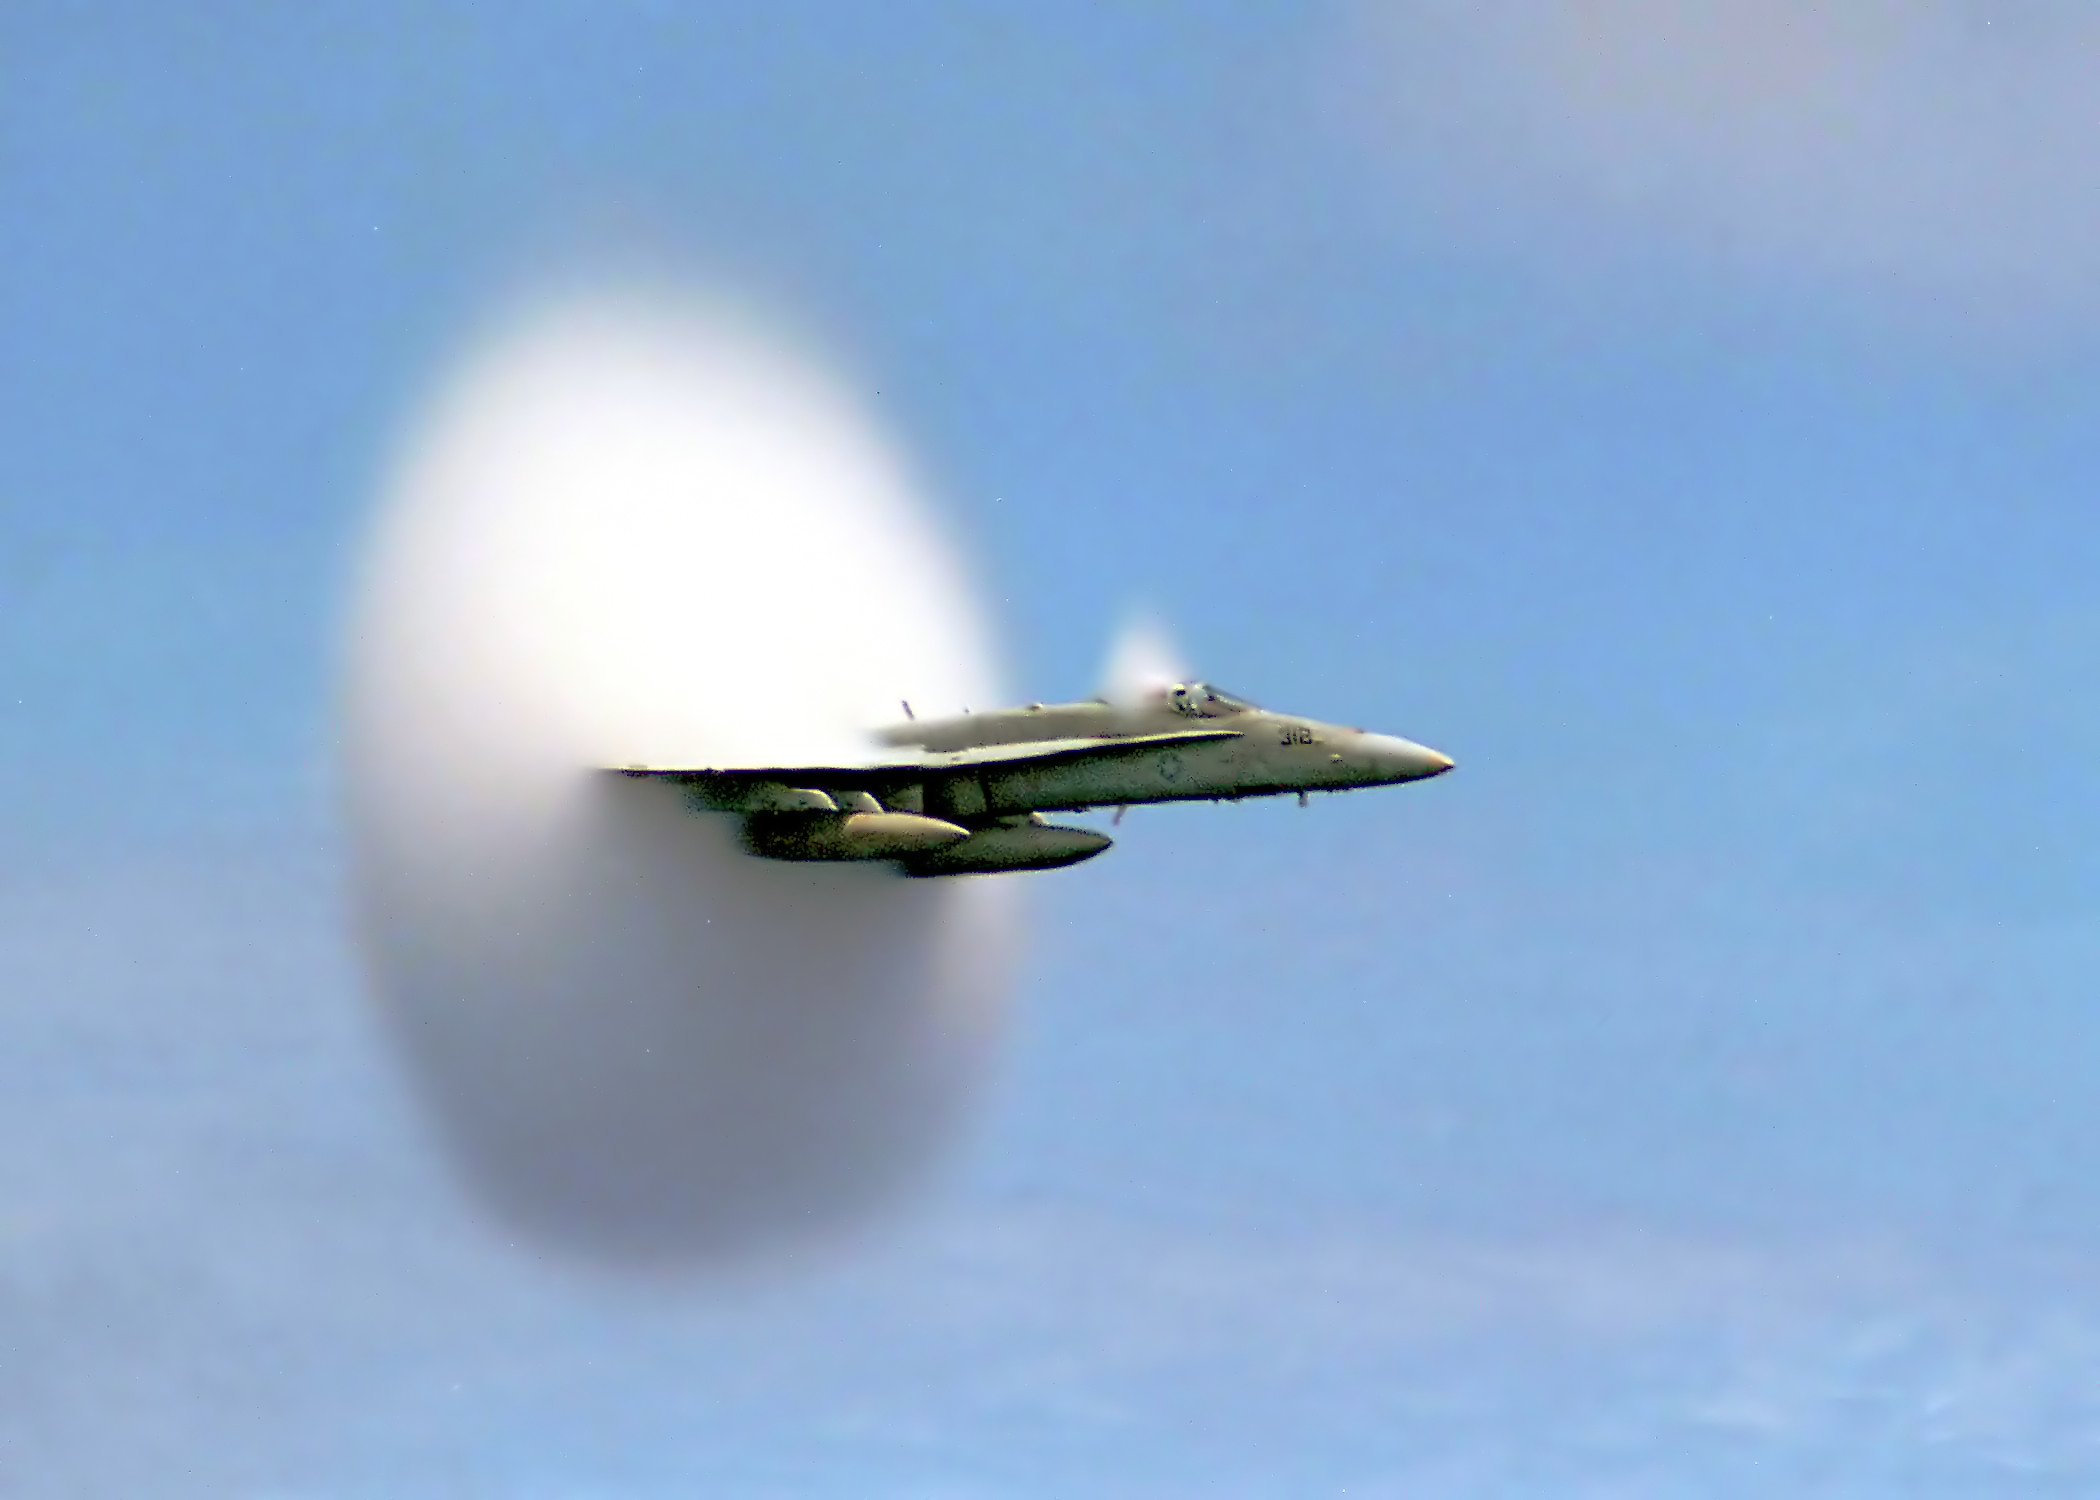
\includegraphics[width=0.6\textwidth]{FA-18_Hornet_breaking_sound_barrier_(7_July_1999)_-_filtered.jpg}
    \caption{Avião caça FA-18 num exercício militar quebrando a barreira do som.}
    \label{fig:barreira do som}
\end{figure}

\section{Intensidade auditiva ($\beta$)}

Uma outra forma usada para analisar intensidade sonora é por meio da \textbf{intensidade auditiva ($\beta$)}. Essa quantidade é definida como:
\begin{equation}
    \beta = 10\,\log_{10}\left(\frac{I}{I_0}\right)
\end{equation}
\noindent em que $I_0$ é a intensidade mínima auditiva: $I_0 = 10^{-12}\frac{W}{m^2}$ e $I$ é a intensidade da onda que ouvimos. \textbf{A intensidade audtiva tem a unidade de decibel $(dB)$}. Em média, sons acima de 120 dB são danosos ao nosso sistema auditivo, podendo até ficarmos surdos. 

Como a fórmula depende do logaritmo da intensidade sonora, para que o som suba por 10 dB, a intensidade sonora ($I$) tem que aumenta por 10 vezes.

Um uso de altos barulhos/sons é usado como forma de atrapalhar os adversários nos mais diversos esportes. Por isso, nos últimos anos, diversos estádios/arenas têm sido construídas de forma que o som vindo das arquibancadas no campo/quadra seja o mais alto possível. 

O recorde mundial atual aconteceu em 2014 no Arrowhead Stadium em Kansas City nos EUA. A torcida do time de futebol americano Kansas City Chiefs fez um barulho de incríveis 142,2 dB durante uma partida de futebol americano. O som é equivalente a estar ao lado de um jato militar, como na foto acima, durante uma decolagem.

\section{Cordas vibrantes e Harmônicos}
Numa corda, podemos fazer diversas configurações de ondas estacionárias, mas sob uma única condição: de que as pontas das cordas não se mexam. Ou seja, para uma corda de comprimento L, em $x=0$ e $x=L$ estão obrigatoriamente 2 nós. Se olharmos uma onda estacionária, vemos que entre 2 nós quaisquer há sempre, pelo menos, um ventre.

Mas pode haver mais do que 1 ventre, pode haver 2, 3, 4 ventres, lembrando sempre que a cada par de ventres também tem um nó. \textbf{Chamamos de harmônico as ondas estacionárias formadas numa corda, em que o número do harmônico é o número de ventres dessa onda estacionária na corda.}

\begin{figure}[H]
    \centering
    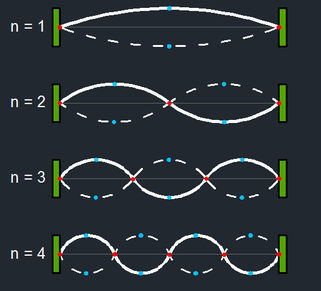
\includegraphics[width=0.6\textwidth]{harmonicos.png}
    \caption{Representação dos harmônicos numa corda}
    \label{fig:harmonicos}
\end{figure}

Chamamos a onda estacionária com um ventre de \textbf{harmônico fundamental ou primeiro harmônico} (n=1). A onda com 2 ventres, chamamos de segundo harmônico (n=2) e assim por diante.

Lembremos da aula passada que a distância entre 2 nós/ventres consecutivos é metade do comprimento de onda ($\lambda/2$). Vemos que, no Harmônico Fundamental. só tem 2 nós (os dos extremos da corda),logo, se a corda tem comprimento L, o comprimento de onda será:
\begin{equation}
    \frac{\lambda}{2}=L \implies \lambda= 2L
\end{equation}

Para o segundo harmônico, temos 3 nós, então:
\begin{equation}
    2\frac{\lambda_2}{2}=L \implies \lambda_2=L
\end{equation}
E assim por diante. Podemos escrever a regra geral para o comprimento de onda do harmônico em relação ao número dele e ao comprimento da corda:
\begin{equation}
    \lambda_n = \frac{2\lambda}{n}
\end{equation}
\noindent em que '$n$' é o número do harmônico.

\begin{figure}[H]
    \centering
    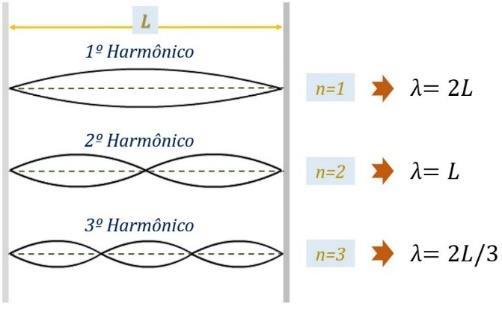
\includegraphics[width=0.6\textwidth]{harmonico_2.jpg}
    \caption{Os primeiros 4 harmônicos com os seus comprimentos de onda}
    \label{fig:harmonico_2}
\end{figure}

Podemos também determinar a frequência do harmônico substituindo o comprimento de onda do harmônico na equação de onda $v=\lambda\,f$.

\section{Harmônicos em tubos}
Uma outra forma de analisar harmônicos e ondas estacionárias é dentro de tubos com extremidades abertas ou fechadas. Mas aqui, temos uma leve diferença: \textbf{caso a extremidade do tubo for aberta, a onda na extremidade será um ventre. Caso a extremidade do tubo for fechada, a onda na extremidade será um nó.}

Com isso, se o tubo for fechado nas 2 pontas, os harmônicos serão idênticos aos da corda, por isso só iremos analisar os harmônicos em tubos abertos nas duas pontas ou aberto numa ponta, mas a outra ponta fechada.

Lembrando que em extremidades abertas, a onda estacionária é um ventre e em extremidades fechadas, a onda estacionária é um nó, temos os seguintes harmônicos em um tubo com uma extremidade aberta e a outra fechada (coluna esquerda) e num tubo com ambas extremidades abertas (coluna direita):
\begin{figure}[H]
    \centering
    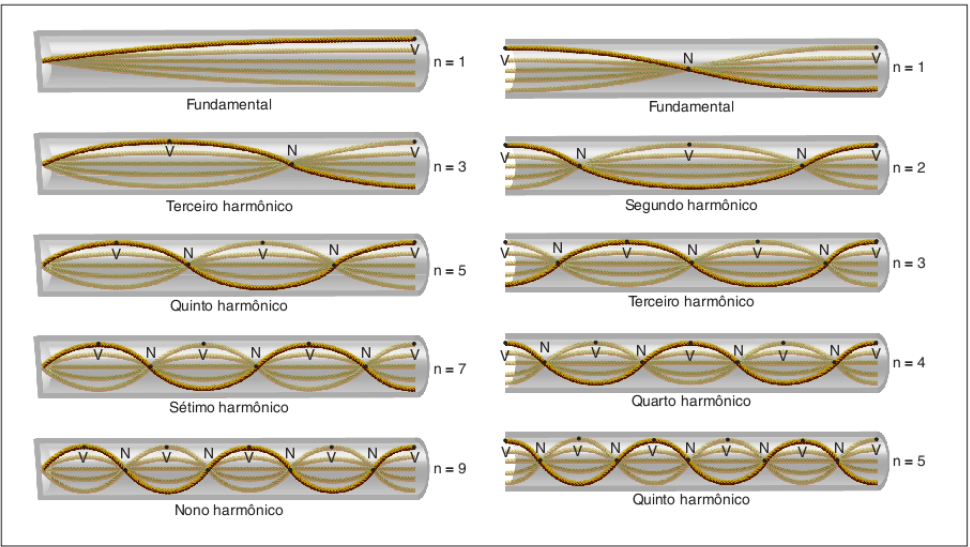
\includegraphics[width=0.9\textwidth]{tubos.png}
    \caption{Harmônicos em tubos com uma extremidade aberta e a outra fechada (coluna esquerda) e com ambas extremidade abertas (coluna direita)}
    \label{fig:tubos}
\end{figure}

Perceba que o Harmônico Fundamental do tubo com uma extremidade fechada e a outra aberta (coluna esquerda) tem um nó e um ventre. Sabemos que a distância entre 2 nós consecutivos é $\lambda/2$ e que o ventre está no meio do caminho entre 2 nós, logo a distância entre um nó e um ventre é $\lambda/4$. Se o tubo tem comprimento L, então:
\begin{equation}
    L= \frac{\lambda}{4} \implies \lambda = 4L
\end{equation}

Para o terceiro harmônico, temos 2 nós e 2 ventres, mas um nó está numa extremdade e um ventre está na outra. Pela figura, vemos que o comprimento do tubo é a soma da distância entre 2 nós e a distância entre um nó. Então:
\begin{equation}
    L = \frac{\lambda}{2}+\frac{\lambda}{4} = \frac{3\lambda}{4} \implies \lambda = \frac{4L}{3}
\end{equation}

Podemos construir uma regra geral para harmônicos em tubos com uma extremidade aberta e a outra fechada:
\begin{equation}
    \lambda_n = \frac{4L}{n}\quad\quad\quad n=1,\,3,\,5,\,7,\,\dots
\end{equation}
Perceba que para esse tipo de tubo, só há harmônicos ímpares. Isso acontece, porque os harmônicos pares não cabem no tubo e não respeitam a regra das extremidades.

Para o tubo com ambas as extremidades abertas, vemos que, para o Harmônico Fundamental, em ambas as extremidades temos ventres. Sabemos que a distância entre 2 ventres é $\lambda/2$ e que o tubo tem tamanho L, logo:
\begin{equation}
    \frac{\lambda}{2}=L \implies\lambda = 2L
\end{equation}
Para o segundo harmônico, vemos que temos 3 ventres, sendo 2 nas extremidades. Como a distância entre 2 ventres consecutivos é $\lambda/2$, então:
\begin{equation}
    2\frac{\lambda}{2}=L \implies \lambda=L
\end{equation}
Também podemos escrever uma regra geral para os harmônicos no tubo de pontas abertas:
\begin{equation}
    \lambda_n = \frac{2L}{n} \quad\quad\quad n=1,\,2,\,3,\,4,\,\dots
\end{equation}
\noindent em que $n$ é o número do harmônico. Perceba que a expressão é a mesma para os harmônicos numa corda. Ou seja, para os harmônicos, é equivalente as pontas serem abertas ou fechadas, desde que ambas sejam abertas ou fechadas.

O mais importante para lembrar de harmônicos é a seguinte frase:
\begin{quote}
    Caso o tubo tenha uma ponta fechada ou a corda tenha a ponta fixa, nessa ponta, a onda estacionária é um nó.
    
    Caso o tubo tenha um ponta aberta ou a corda tenha a ponta presa a um suporte móvel, a onda estacionária é um ventre.
\end{quote}

A partir dessas afirmações, podemos desenhar e deduzir os harmônicos de uma tubo ou de uma corda, precisando somente saber qual é o tamanho dessa corda/tubo.

\section{Efeito Doppler}

Damos o nome de Efeito Doppler o fenômeno de mudança da frequência da onda/som devido ao movimento da fonte em relação ao observador. Isso acontece mais perceptivelmente na Fórmula 1, em que o ronco do motor é mais agudo conforme o carro se aproxima da gente e mais grave, conforme o carro se afasta. O mesmo acontece para a sirene de ambulâncias e carros de polícia.

A fórmula do Efeito Doppler é dado por:
\begin{equation}
    f_{aparente} = \left(\frac{v_{s} \pm v_{obs}}{v_s \mp v_{fonte} }\right)f
\end{equation}
\noindent em que $f$ é a frequência da onda gerada pela fonte, $v_{obs}$ é a velocidade do observador, $v_{fonte}$ é a velocidade da fonte e $v_s$ é a velocidade de propagação do som (normalmente $v_s=343\,m/s$).

\textbf{Uma questão importante e que muita gente se confunde: usamos os sinais de cima para o caso em que a fonte se aproxima do observador e usamos os sinais de baixo para o caso em que a fonte se afasta do observador.}

Para fonte se aproximando:
\begin{equation}
     f_{aparente} = \left(\frac{v_{s} + v_{obs}}{v_s - v_{fonte} }\right)f
\end{equation}
Para fonte se afastando:
\begin{equation}
     f_{aparente} = \left(\frac{v_{s} - v_{obs}}{v_s + v_{fonte} }\right)f
\end{equation}

Esse efeito é muito usado em técnicas de medição astronômicas para calcular órbitas de galáxias muito distantes da gente. Caso a galaxia se aproxima da gente, a luz da galaxia tende a luz azul, ao fenômeno, damos o nome de \textit{blueshift}. Caso a galaxia se afasta da gente, a luz dela tende à luz vermelha, assim damos ao fenômeno o nome de \textit{redshift}.

\begin{figure}[H]
    \centering
    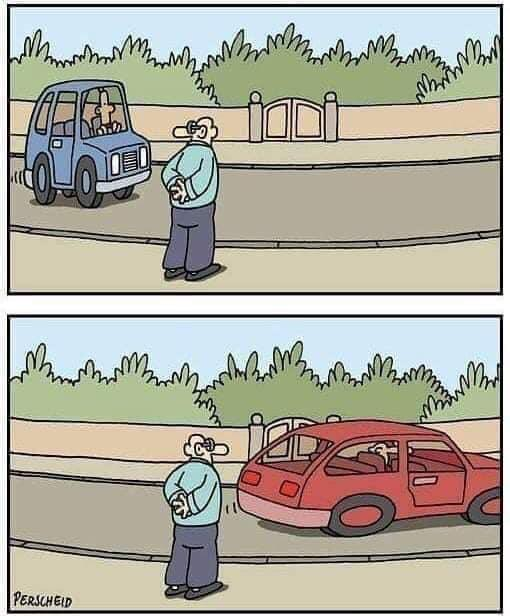
\includegraphics[width=0.6\textwidth]{red_blueshift_meme.jpg}
    \caption{Uma charge/meme do fenômeno de red/blueshift. O carro anda tão rápido que a cor dele muda de azul (quando ele se aproxima) para vermelho quando ele se afasta por causa do Efeito Doppler.}
    \label{fig:red_blueshift_meme}
\end{figure}

\end{document}
